\documentclass{article}
\usepackage{graphicx}
\usepackage{wrapfig}
\usepackage{filecontents}
\usepackage{siunitx}
\usepackage[table]{xcolor}
\usepackage{float}
\usepackage{hyperref}

\usepackage{color} % balíček pro obarvování textů
\usepackage{xcolor}  % zapne možnost používání barev, mj. pro \definecolor
\usepackage{pgfplots} % http://www.chiark.greenend.org.uk/doc/texlive-doc/latex/pgfplots/pgfplots.pdf

\ifnum 0\ifxetex 1\fi\ifluatex 1\fi=0 % if pdftex
  \usepackage[T1]{fontenc}
  \usepackage[utf8]{inputenc}
\else % if luatex or xelatex
  \ifxetex
    \usepackage{mathspec}
  \else
    \usepackage{fontspec}
  \fi
  \defaultfontfeatures{Ligatures=TeX,Scale=MatchLowercase}
\fi
\usepackage[total={175mm,230mm}, top=23mm, left=20mm, includefoot]{geometry}
\hypersetup{
    colorlinks,
    linkcolor={blue!50!black},
    citecolor={green!50!black},
    urlcolor={blue!80!black}
}
\definecolor{orange}{RGB}{ 251, 114, 032}
\definecolor{fialova}{RGB}{ 255, 000, 255}

\newcommand \obr[1]
{ obr. \ref{#1}}

\newcommand \tab[1]
{ tab. \ref{#1}}

\begin{document}

\section*{Laboratorní cvičení č. 2 – Měření napětí - stejnosměrné a~střídavé voltmetry}

\textbf{
    \begin{itemize}
        \item Autor: Tomáš Vavrinec
        \item Datum měření: 3.10.2022
    \end{itemize}
}

\subsection*{Úkoly}

\begin{enumerate}
    \item Pomocí referenčního multimetru Agilent34401A ověřte přesnost voltmetru laboratorního zdroje GWInstek GPD-3303S v~rozsahu 0 až 10 v~DC s~krokem měření 1V. Vypočtěte absolutní a~relativní chyby měření stejnosměrného napětí, korekci K a~vykreslete korekční křivku, za předpokladu, že správné hodnoty napětí udává multimetr Agilent 34401A.
    \item Změřte vstupní odpor Rvst multimetru Keysight 34450A na rozsahu 10 v~DC a~vstupní odpor Rvst multimetru Agilent (HP) 34401A na rozsahu 1 v~DC pomocí napěťového děliče. Jako zdroj ss. napětí použijte funkční generátor Siglent SDG2042X. Naměřené hodnoty porovnejte s~údajem od výrobce.
    \item Změřte frekvenční charakteristiky multimetrů Keysight 34450A a~Agilent 34401A pro sinusový signál z~generátoru Siglent SDG 2042X s~amplitudou 1,5 v~v~rozsahu 1 kHz až 500 kHz (zvolit minimálně 10 hodnot). Dosažené výsledky graficky zakreslete. Zhodnoťte dosažené výsledky měření na základě informací o~frekvenčním rozsahu multimetrů zjištěných ze specifikace přístroje.
    \item Multimetrem Keysight 34450A změřte efektivní hodnotu výstupních signálů, jejichž zdrojem je generátor Siglent SDG 2042X:
    \begin{itemize}
        \item Obdélníkový průběh, f =1 kHz, Up-p=3 V
        \item Trojúhelníkový průběh, f =100 Hz, Up-p=5 V
    \end{itemize}
    Průběhy signálů zakreslete do sešitu a~popište.
    Ověřte výpočtem velikosti efektivních hodnot uvedených signálů, vypočtěte absolutní a~relativní chybu měření (správnou hodnotou je hodnota vypočtená) a~dosažené výsledky zhodnoťte.
    Určete velikost absolutních a~relativních chyb údaje multimetru Keysight 34450A pro tato měření.
    \item U číslicového multimetru Agilent 34401A ve funkci stejnosměrného voltmetru s~nastavením rozlišení 4digit/slow a~5digit/slow změřte na rozsahu 1V závislost činitele potlačení sériového rušení H na frekvenci fr rušivého napětí. Frekvenci volte v~rozsahu fr = 45 až 55 Hz po kroku 1 Hz u rozlišení 4digit/slow a~po kroku 0,5 Hz u rozlišení 5digit/slow. Hodnota napětí Uss je nulová (pro zjednodušení).
\end{enumerate}

\section*{Příprava}
Nejčastější měření v~elektrotechnice je měření napětí.
Voltmetry mohou být rozděleny podle:

\begin{figure}[H]
    \scriptsize
    {
        \begin{minipage}[t]{0.24\textwidth}
            1) způsobu měření
            \begin{itemize}
                \item analogové
                \item číslicové (digitální).
            \end{itemize}
        \end{minipage}
        \hfill
        \begin{minipage}[t]{0.24\textwidth}
            2) podle druhu měřeného napětí:
            \begin{itemize}
                \item stejnosměrné
                \item střídavé
                \item impulsní
            \end{itemize}
        \end{minipage}
        \hfill
        \begin{minipage}[t]{0.24\textwidth}
            3) podle citlivosti
            \begin{itemize}
                \item voltmetry
                \item milivoltmetry
                \item mikrovoltmetry
                \item nanovoltmetry.
            \end{itemize}
        \end{minipage}
        \hfill
        \begin{minipage}[t]{0.24\textwidth}
            4) podle kmitočtové oblasti (střídavé voltmetry):
            \begin{itemize}
                \item nízkofrekvenční
                \item vysokofrekvenční
                \item širokopásmové
                \item selektivní (úzkopásmové)
            \end{itemize}
        \end{minipage}
    }
\end{figure}

\newpage
\subsection*{Korekční křivka}
\begin{wrapfigure}{r}{0.5\textwidth}
    % \centering
    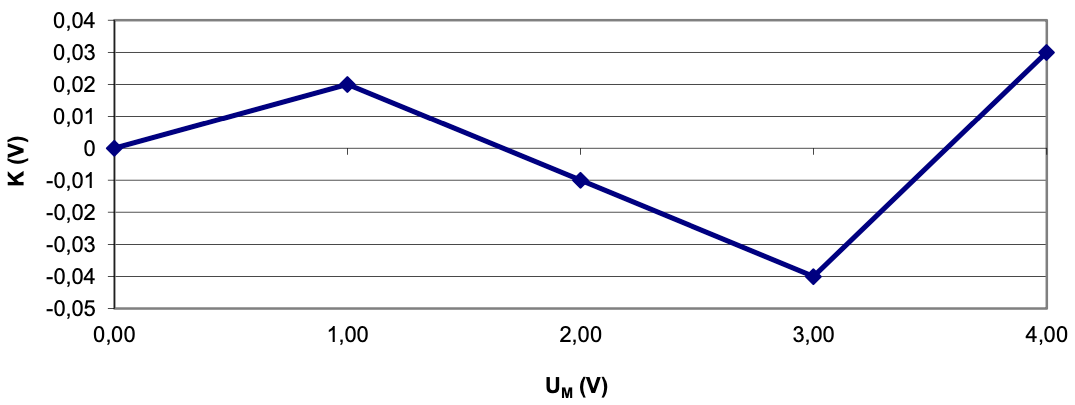
\includegraphics[width=0.55\textwidth]{obrazky/korekcni_krivka.png}
    \caption{\label{korek_krivka}Příklad korekční křivky}
\end{wrapfigure}
Pokud chceme zvýšit přesnost měření konkrétního přístroje, můžeme k jeho měření přičítat hodnotu z~korekční křivky.
Korekční křivku můžeme získat porovnáním měření s~přesnějším přístrojem (etalonem) \(k = -\delta_x = X_S X_M\), kde \(X_S\) je hodnota naměřena na etalonu a~\(X_M\) je hodnota naměřena na kontrolovaném přístroji.

\subsection*{Vstupní odpor voltmetru}
\begin{wrapfigure}{r}{0.48\textwidth}
    \vspace{-10mm}
    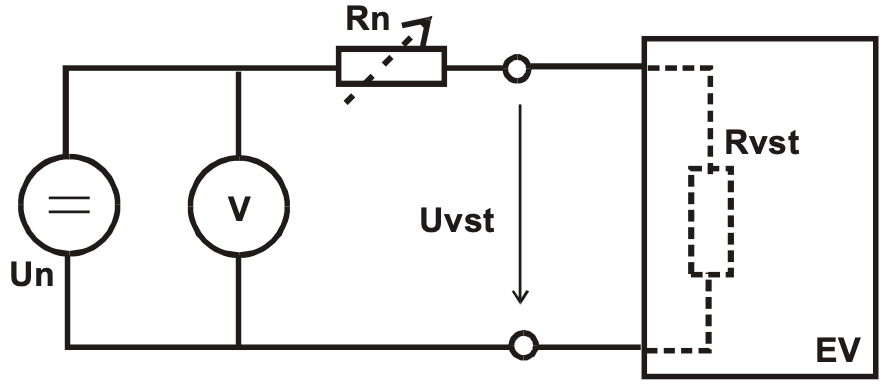
\includegraphics[width=0.52\textwidth]{obrazky/vstup_odpor.png}
    \caption{\label{vstupni_odpor}Zapojení pro měření vstupního odporu voltmetru}
\end{wrapfigure}
Vstupní odpor voltmetru je odpor, který je mezi \\vstupními vodiči.
Dá se jednoduše určit pomocí zdroje napětí a~rezistoru se srovnatelným odporem.
\(R_{vst}=\frac{U_{vst}}{U_{n}-U_{vst}}\cdot R_n\)

\subsection*{Měření AC}
Běžný frekvenční rozsah se pohybuje od \(100\-kHz\) \\do \(1\-MHz\).
Jeden z~parametrů AC voltmetru je způsob měření efektivní hodnoty.
Buď měřený signál usměrní, změří jeho střední hodnotu a~převede ji na efektivní, tato metoda je však přesná jen pro harmonický signál (střední hodnota se násobí konstantou, která souvisí s~konkrétním tvarem signálu a~pochopitelně se proto používá nejběžnější tvar).
Druhá možnost je signál měřit pomocí definice efektivní hodnoty, která je vypočítána takto:
\begin{equation}
    U_{efe} = \sqrt{\frac{1}{T}\int_{0}^{T}U^2(t)dt}
    \label{proud_kolektoru}
\end{equation}

\subsection*{Chyby měření}
Absolutní chyba měřícího přístroje se dá spočítat jako:

\begin{figure}[H]
    \begin{equation}
        |\Delta_{Px}| = |\Delta_{M}|+|\Delta_{R}| = \frac{|\delta_M\cdot X_M|+|\delta_R\cdot X_R|}{100}
    \end{equation}
    \caption{\label{proud_kolektoru}Jednotka veličiny X}
\end{figure}
Chyba měření může vzniknout také sériovým rušením, které je způsobeno především rušením ze sítě (\(50\-Hz\)), toto rušení integrační AD převodníky z~principu potlačují.
Potlačení rušení se dosahuje integrací v~časovém úseku, který je celočíselným násobkem periody měřeného napětí, pro (\(50\-Hz\)) je to \(20\-ms\).

Činitel potlačení sériového rušení je definován vztahem:
\begin{figure}[H]
    \begin{equation}
        H = 20 \cdot \log_{10}\frac{U_{rm}}{\Delta U_{ch}}\-[dB]
    \end{equation}
    \caption{\label{cinitel_potlaceni} Činitel potlačení sériového rušení}
\end{figure}
Kde \(U_{rm}\) je amplituda rušivého signálu a~\(U_{ch}\) je chyba měření vyvolaná rušivým napětím.


\section*{Měření}
\subsection*{Použité přístroje}
\begin{itemize}
    \item Multimetr Keysight 34450A
    \item Multimetr Agilent 34401A
    \item Stabilizovaný zdroj napětí GW Instek GPD-3303S Generátor Siglent SDG2042X
    \item Odporová dekáda
\end{itemize}

\subsection*{Úkol 1}
\begin{figure}[H]
    \begin{minipage}[t]{0.4\textwidth}
        \begin{table}[H]
            % \vspace{-75mm}
            \begin{tabular}{|c|c|c|c|}
            \hline
                \(U_{GWI}\)        &	\(U_{AGI}\)            &	\(K\)        & \(\delta_U\)       \\ \hline
                \(V\)              &    \(V\)                  &	\(mV\)              & \(\%\) \\ \hline
                 0.0               &    0.0007	               &    -0.7                & -0.07 \\ \hline
                 1.0               &    1.0044	               &    -4.4                & -0.44 \\ \hline
                 2.0               &    2.0042	               &    -4.2                & -0.42 \\ \hline
                 3.0               &    3.0038	               &    -3.8                & -0.38 \\ \hline
                 4.0               &    4.0036	               &    -3.6                & -0.36 \\ \hline
                 5.0               &    5.0034	               &    -3.4                & -0.34 \\ \hline
                 6.0               &    6.0044	               &    -4.4                & -0.44 \\ \hline
                 7.0               &    7.0041	               &    -4.1                & -0.41 \\ \hline
                 8.0               &    8.0036	               &    -3.6                & -0.36 \\ \hline
                 9.0               &    9.0047	               &    -4.7                & -0.47 \\ \hline
                10.0               &    10.0044                &	-4.4                & -0.44 \\ \hline
            \end{tabular}
            \caption{\label{tab_pracovni_bod} Nastavení obvodu}
        \end{table}
    \end{minipage}
    \hfill
    \begin{minipage}[t]{0.6\textwidth}
        \vspace{-10mm}
        \begin{tikzpicture}
            \hspace{-10mm}
            \begin{axis}[
                title={korekční křivka voltmetru GWInstek GPD-3303S},
                xlabel={\(U_{mer}~[V]\)},
                ylabel={\(K~[mV]\)},
                xmin=0, xmax=10,
                ymin=0, ymax=5,
                legend pos=north west,
                width=1.1\textwidth, 
                height=80mm,
            ]
            \addplot[
                color=green,
                mark=x,
                ]
                coordinates {
                        ( 0.0 ,0.7)
                        ( 1.0 ,4.4)
                        ( 2.0 ,4.2)
                        ( 3.0 ,3.8)
                        ( 4.0 ,3.6)
                        ( 5.0 ,3.4)
                        ( 6.0 ,4.4)
                        ( 7.0 ,4.1)
                        ( 8.0 ,3.6)
                        ( 9.0 ,4.7)
                        (10.0 ,4.4)
                    };
            \addlegendentry{\scriptsize}
            \end{axis}
        \end{tikzpicture}
    \end{minipage}
\end{figure}

\vspace{5mm}
\(
    GWInstek GPD-3303S ... U_{GWI}
\)
\\
\vspace{5mm}
\(
    Agilent 34401A      ... U_{AGI}
\)\\
\vspace{5mm}
Příklad výpočtu Absolutní odchylka: 
\(
    \Delta_U = U_{GWI} - U_{AGI} = (1 - 1.0044)\-[V]= -0.0044\-[V]
\)\\
\vspace{5mm}
Příklad výpočtu Relativní odchylka: \(
    \Delta_U = \frac{U_{GWI} - U_{AGI}}{U_{GWI}}\cdot100 = \frac{1 - 1.0044}{1}\cdot100 = -0.44\-[\%]
\)\\
\vspace{5mm}
Střední odchylku můžeme určit jako:
\(
    \Delta_{str} = \Sigma_{i=1}^{n}\frac{\Delta_{Ui}}{n} = \Sigma_{i=1}^{11}\frac{\Delta_{Ui}}{11} = \frac{0.7 + 4.4 + 4.2 + ... 4.4}{11} = 3.8\-[mV]
\)

\subsection*{Úkol 2}

\begin{figure}[H]
    \begin{minipage}[t]{0.3\textwidth}
        \subsubsection*{Agilent 34401A}
        \begin{itemize}
            \item \(R_n = 100\-k\Omega\) 
            \item \(U_n = 1.0032\-V\) 
            \item \(U_{vstup} = 0.9933\-V\) 
        \end{itemize}
    \end{minipage}
    \hfill
    \begin{minipage}[t]{0.7\textwidth}
        \vspace{10mm}
        \(
            R_{vst} = \frac{U_{vst}}{U_{n}-U_{vst}}\cdot R_n = \frac{0.9933}{1.0032-0.9933}\cdot 100*10^3 = 10.033\-[M\Omega]  
        \)
    \end{minipage}
\end{figure}
Podle katalogového listu přístroje Agilent 34401A je jeho vstupní odpor \(10\-M\Omega \)\\odchylka našeho měření je tady \(33\-k\Omega\)

\begin{figure}[H]
    \begin{minipage}[t]{0.3\textwidth}
        \subsubsection*{Keysight 34450A}
        \begin{itemize}
            \item \(R_n = 100\-k\Omega\) 
            \item \(U_n = 1.0027\-V\) 
            \item \(U_{vstup} = 0.9928\-V\) 
        \end{itemize}
    \end{minipage}
    \hfill
    \begin{minipage}[t]{0.7\textwidth}
        \vspace{10mm}
        \(
            R_{vst} = \frac{U_{vst}}{U_{n}-U_{vst}}\cdot R_n = \frac{0.9928}{1.0027-0.9928}\cdot 100*10^3 = 10.028\-[M\Omega]  
        \)
    \end{minipage}
\end{figure}
Podle katalogového listu přístroje Keysight 34450A je jeho vstupní odpor \(10\-M\Omega \)\\odchylka našeho měření je tady \(28\-k\Omega\)

\subsection*{Úkol 3}
Pomocí generátoru jsme vytvářeli harmonický signál o~amplitudě \(1\-[V]\), kterému jsme měnili frekvenci v~rozsahu \(1\-[kHz]\)-\(500\-[kHz]\).\\ 
\begin{table}[H]
    \footnotesize
    \vspace{-6mm}
    \hspace{-8mm}
    \begin{tabular}{|c|c|c|c|c|c|c|c|c|c|c|}
    \hline
                        & 1 [kHz]  	& 2 [kHz]	& 5 [kHz]	& 10 [kHz]	& 20 [kHz]	& 50 [kHz]	& 100 [kHz]	& 200 [kHz]	& 350 [kHz]	& 500 [kHz] \\ \hline
    Silent SDG 2042 [V]	& 1	        & 1	        & 1      	& 1   	    & 1   	    & 1   	    & 1   	    & 1	        & 1   	    & 1         \\ \hline
    Agilent 34401A  [V] & 1,05932	& 1,0537	& 1,05556	& 1,05977	& 1,05920	& 1,05441	& 1,04235	& 1,0158	& 0,9250	& 0,71208   \\ \hline
    Keysight 34450A [V]	& 1,0588	& 1,0589	& 1,0591	& 1,0592	& 1,0592	& 1,0576	& 1,0536	& 1,0464	& 1,0341	& 1,0186    \\ \hline
    \end{tabular}
    \caption{\label{frekvencni_rozsah} Měření frekvenčního rozsahu}
    \normalsize
\end{table}

\pgfplotsset{width=100mm,compat=1.9}
\begin{tikzpicture}
    \hspace{-10mm}
    \begin{semilogxaxis}[
        title={Odchylka měření v~závislosti na frekvenci měřeného signálu},
        width=0.925\textwidth, 
        height=100mm,
        xlabel={\(f~[kHz]\)},
        ylabel={\(U_{mer}~[V]\)},
        xmin=1, xmax=500,
        ymin=0.7, ymax=1.1,
        legend pos=south west,
    ]
    \addplot[
        only marks,
        color=green,
        mark=x,
        ]
        coordinates {
                ( 1   ,1.05932)
                ( 2   ,1.0537)
                ( 5   ,1.05556)
                ( 10  ,1.05977)
                ( 20  ,1.05920)
                ( 50  ,1.05441)
                ( 100 ,1.04235)
                ( 200 ,1.0158)
                ( 350 ,0.9250)
                ( 500 ,0.71208)
            };
    \addlegendentry{\scriptsize Agilent 34401A}
    \addplot[
        only marks,
        color=red,
        mark=x,
        ]
        coordinates {
                ( 1   ,1.0588)
                ( 2   ,1.0589)
                ( 5   ,1.0591)
                ( 10  ,1.0592)
                ( 20  ,1.0592)
                ( 50  ,1.0576)
                ( 100 ,1.0536)
                ( 200 ,1.0464)
                ( 350 ,1.0341)
                ( 500 ,1.0186)
            };
    \addlegendentry{\scriptsize Keysight 34450A}
    \addplot[
        color=blue,
        ]
        coordinates {
                ( 0.1,1)
                ( 550,1)
            };
    \addlegendentry{\scriptsize Silent SDG 2042}
    \addplot[
        color=green,
        ]
        coordinates {
                ( 1   ,1.05932)
                ( 2   ,1.0537)
                ( 5   ,1.05556)
                ( 10  ,1.05977)
                ( 20  ,1.05920)
                ( 50  ,1.05441)
                ( 100 ,1.04235)
                ( 150 ,1.03)
                ( 200 ,1.0158)
                ( 245 ,0.995)
                ( 300 ,0.96)
                ( 350 ,0.9250)
                ( 400 ,0.88)
                ( 450 ,0.81)
                ( 500 ,0.71208)
            };
    \addplot[
        color=red,
        ]
        coordinates {
                ( 1   ,1.0588)
                ( 2   ,1.0589)
                ( 5   ,1.0591)
                ( 10  ,1.0592)
                ( 20  ,1.0592)
                ( 50  ,1.0576)
                ( 100 ,1.0536)
                ( 200 ,1.0464)
                ( 280 ,1.04)
                ( 350 ,1.0341)
                ( 430 ,1.026)
                ( 500 ,1.0186)
            };
    \end{semilogxaxis}
\end{tikzpicture}
Katalogový frekvenční rozsah multimetru Agilent 34401A je \(300\-[kHz]\), ale chyba jeho měření je dle našeho měření menší jak \(0.1\-[V]\) i při frekvenci \(300\-[kHz]\), u vyšších frekvencí pak přesnost rychle padá.
U multimetru Keysight 34450A jsme naměřili odchylku měření menší jak \(0.1\-[V]\) i při frekvence \(500\-[kHz]\).

\newpage
\subsection*{Úkol 4}
Multimetrem Keysight 34450A jsme změřili nejprve obdélníkový (\(U_{pp} = 3\-[V]\);\(f=1\-[kHz]\)) signál a~následně trojúhelníkový (\(U_{pp} = 5\-[V]\);\(f=100\-[Hz]\))
\begin{itemize}
    \item obdélníkový signál - \(U_{EF} = 1.4850\-[V]\)
    \item trojúhelníkový signál - \(U_{EF} = 1.4411\-[V]\)
\end{itemize}

\begin{figure}[H]
    \begin{minipage}[t]{0.7\textwidth}
        \vspace{-55mm}
        \hspace{-5mm}
        Elektivní hodnota obdélníkového signálu (\(U_{pp} = 3\-[V]\);\(f=1\-[kHz]\)) je:
        \\
        \(
            U_{EF} = \sqrt{\frac{1}{T}(\int_{0}^{T}U^2(t)dt} = \\
            = \sqrt{\frac{1}{\frac{1}{1000\-[Hz]}}\Biggl(\int_{0}^{\frac{\frac{1}{1000\-[Hz]}}{2}}1.5^2dt+\int_{0}^{\frac{\frac{1}{1000\-[Hz]}}{2}}(-1.5)^2dt\Biggl)} = \\\
            = \sqrt{1000\cdot2\int_{0}^{0.0005}2.25dt} =\\
            = \sqrt{1000\cdot2\cdot\bigr[2.25t \bigr]_{0}^{0.0005}} = \sqrt{1000\cdot2\cdot0.001125} = 1.5\-[V]
        \)
        \\
        Měření tedy oproti teorii vykazuje odchylku \(15\-[mV]\)
    \end{minipage}
    \hfill
    \begin{minipage}[t]{0.4\textwidth}
        \hspace{-5mm}
        \pgfplotsset{width=\textwidth,compat=1.9}
        \begin{tikzpicture}
            \begin{axis}[
                title={obdelníkový signál},
                xlabel={\(t~[ms]\)},
                ylabel={\(U~[V]\)},
                xmin=0, xmax=2.5,
                ymin=-2, ymax=2,
                legend pos=south west,
            ]
            \addplot[
                color=green,
                ]
                coordinates {
                        (0   ,-1.5)
                        (0.5 ,-1.5)
                        (0.5 , 1.5)
                        (1   , 1.5)
                        (1   ,-1.5)
                        (1.5 ,-1.5)
                        (1.5 , 1.5)
                        (2   , 1.5)
                        (2   ,-1.5)
                        (2.5 ,-1.5)
                    };
            \end{axis}
        \end{tikzpicture}
    \end{minipage}
\end{figure}

\begin{figure}[H]
    \begin{minipage}[t]{0.7\textwidth}
        \vspace{-60mm}
        \hspace{-5mm}
        Elektivní hodnota trojúhelníkového signálu (\(U_{pp} = 5\-[V]\);\(f=100\-[Hz]\)) je: \\
        \(
            U_{EF} = \sqrt{\frac{1}{T}(\int_{0}^{T}U^2(t)dt} = \\
            = \sqrt{\frac{1}{\frac{1}{100\-[Hz]}}\Biggl(\int_{0}^{\frac{\frac{1}{100\-[Hz]}}{2}} (-2.5+1000t)^2 dt+\int_{\frac{\frac{1}{100\-[Hz]}}{2}}^{\frac{1}{100\-[Hz]}} (7.5-1000t)^2 dt\Biggl)} = \\
            = \sqrt{100\cdot\Biggl(\int_{0}^{0.005} 6.25-5000t+10^6t^2 dt + \int_{0.005}^{0.01} 56.25-15000t+10^6t^2 dt\Biggl)} = \\
            = \sqrt{100\cdot\Bigr(\bigr[6.25t-2500t^2+\frac{10^6t^3}{3} \bigr]_{0}^{0.005} + \bigr[56.25t-7500t^2+\frac{10^6t^3}{3}\bigr]_{0.005}^{0.01}\Bigr)} = \\
            = \sqrt{100\cdot(0.01042+0.01042)} = 1.4436\-[V]
        \)
        \\
        Měření tedy oproti teorii vykazuje odchylku \(2.5\-[mV]\)
    \end{minipage}
    \hfill
    \begin{minipage}[t]{0.4\textwidth}
        \hspace{-5mm}
        \pgfplotsset{width=\textwidth,compat=1.9}
        \begin{tikzpicture}
            \begin{axis}[
                title={obdelníkový signál},
                xlabel={\(t~[ms]\)},
                ylabel={\(U~[V]\)},
                xmin=0, xmax=40,
                ymin=-3, ymax=3,
                legend pos=south west,
            ]
            \addplot[
                color=green,
                ]
                coordinates {
                        (00   ,-2.5)
                        (10   , 2.5)
                        (20   ,-2.5)
                        (30   , 2.5)
                        (40   ,-2.5)
                        (50   , 2.5)
                    };
            \end{axis}
        \end{tikzpicture}
    \end{minipage}
\end{figure}

\newpage
\subsection*{Úkol 5}
Jako zdroj rušivého signálu jsme použili zdroj Siglent SDG2042X.
Signál jsme nastavili \(U_{šš} = 1\-[V]\) a~frekvence v~rozsahu \(f = 45-55\-[Hz]\).
Poprvé jsme měřili DC s~potlačením rušení na multimetru Agilent 34401A s~nastavením \(4\-digit/slow\) s~krokem \(1\-[Hz]\) a~podruhé \(5\-digit/slow\) s~krokem \(0.5\-[Hz]\).
Nastavení (Shift + On/Off (tlačítko <) → A: MEAS MENU → 5: RESOLUTION → SLOW 4 Digit), pohyb v~menu je možný šipkami, doprava/doleva, pohyb na stejné úrovni a~nahoru/dolu, zanořování/vynořování z~menu.

\subsubsection*{\(4\-digit/slow\)}
\begin{table}[H]
    \footnotesize
    % \vspace{-6mm}
    \hspace{-10mm}
    \begin{tabular}{|c|c|c|c|c|c|c|c|c|c|c|c|}
    \hline
    \(f\-[Hz]\)                     & 45        & 46	    & 47	    & 48	    & 49	    & 50	    & 51	    & 52	    & 53	    & 54        & 55        \\ \hline
    \(U_{min}\-[mV]\) 	            & -58.85915 & -47.24265 & -35.94526 & -25.00425 & -14.42704 & -4.25088  & -14.04514 & -23.42666 & -32.3752  & -40.8929  & -48.95002 \\ \hline
    \(U_{max}\-[mV]\)	            & 50.39674	& 38.76532	& 27.48497	& 16.54395	& 5.96569	& -4.21890	& 5.555070  & 14.93445	& 23.88194	& 32.38476  & 40.44185  \\ \hline
    \(H\-[db]\)                     & 13.21     & 15.29		& 17.93	   	& 21.6		& 27.79		& 83.88		& 28.13		& 22.30		& 18.98		& 16.68		& 14.95     \\ \hline
    \end{tabular}
    \caption{\label{potlaceni_ruseni} Měření potlačení ručení}
    \normalsize
\end{table}

Příklad výpočtu činitele potlačení
\(
    H = 20 \cdot \log\frac{U_{rm}}{U_{max}-U_{nim}} = 20 \cdot \log\frac{0.5\-[V]}{50.39674\-[mV]- -58.85915\-[mV]} = \\
    = 20\cdot\log4.5764123106 = 20 \cdot 0.66052514518 = 13.2105029038\-[dB]
\)
\\
\begin{figure}[H]
    \begin{minipage}[t]{0.7\textwidth}
        % \hspace{-5mm}
        \pgfplotsset{width=\textwidth,compat=1.9}
        \begin{tikzpicture}
            \begin{axis}[
                title={obdelníkový signál},
                xlabel={\(f~[Hz]\)},
                ylabel={\(U~[mV]\)},
                xmin=45, xmax=55,
                ymin=-60, ymax=60,
                % xtick={45,47.5,50,52.5,55},
                legend pos=south west,
            ]
            \addplot[
                    only marks,
                    color=green,
                    mark = x,
                ]
                coordinates {
                    (45 , 50.39674)
                    (46 , 38.76532)
                    (47 , 27.48497)
                    (48 , 16.54395)
                    (49 , 5.965690)
                    (50 , -4.21890)
                    (51 , 5.555070)
                    (52 , 14.93445)
                    (53 , 23.88194)
                    (54 , 32.38476)
                    (55 , 40.44185)
                    };
                \addlegendentry{\scriptsize \(U_{max}\)}
            \addplot[
                    only marks,
                    color=red,
                    mark = x,
                ]
                coordinates {
                    (45 , -58.85915)
                    (46 , -47.24265)
                    (47 , -35.94526)
                    (48 , -25.00425)
                    (49 , -14.42704)
                    (50 , -4.250880)
                    (51 , -14.04514)
                    (52 , -23.42666)
                    (53 , -32.37520)
                    (54 , -40.89290)
                    (55 , -48.95002)
                    };
                \addlegendentry{\scriptsize \(U_{min}\)}
            \addplot[
                    color=green,
                ]
                coordinates {
                    (45 , 50.39674)
                    (46 , 38.76532)
                    (47 , 27.48497)
                    (48 , 16.54395)
                    (49 , 5.965690)
                    (50 , -4.21890)
                    (51 , 5.555070)
                    (52 , 14.93445)
                    (53 , 23.88194)
                    (54 , 32.38476)
                    (55 , 40.44185)
                    };
            \addplot[
                    color=red,
                ]
                coordinates {
                    (45 , -58.85915)
                    (46 , -47.24265)
                    (47 , -35.94526)
                    (48 , -25.00425)
                    (49 , -14.42704)
                    (50 , -4.250880)
                    (51 , -14.04514)
                    (52 , -23.42666)
                    (53 , -32.37520)
                    (54 , -40.89290)
                    (55 , -48.95002)
                    };
            \end{axis}
            \begin{axis}[
                axis y line*=right,
                title={obdelníkový signál},
                xlabel={\(f~[Hz]\)},
                ylabel={\(H\-[db]\)},
                xmin=45, xmax=55,
                ymin=0, ymax=100,
                legend pos=south east,
            ]
            \addplot[
                    only marks,
                    color=blue,
                    mark = x,
                ]
                coordinates {
                    (45   , 13.21)
                    (46   , 15.29)
                    (47   , 17.93)
                    (48   , 21.60)
                    (49   , 27.79)
                    (50   , 83.88)
                    (51   , 28.13)
                    (52   , 22.30)
                    (53   , 18.98)
                    (54   , 16.68)
                    (55   , 14.95)
                    };
                \addlegendentry{\scriptsize \(K\)}
            \addplot[
                    color=blue,
                ]
                coordinates {
                    (45   , 13.21)
                    (46   , 15.29)
                    (47   , 17.93)
                    (48   , 21.60)
                    (48.5 , 24.3)
                    (49   , 27.79)
                    (49.25, 30.8)
                    (49.5 , 36)
                    (49.6 , 40)
                    (49.75, 50)
                    (49.875, 60)
                    (50   , 83.88)
                    (50.125, 60)
                    (50.25, 50)
                    (50.4 , 40)
                    (50.5 , 36)
                    (50.75, 30.8)
                    (51   , 28.13)
                    (51.5 , 24.3)
                    (52   , 22.30)
                    (53   , 18.98)
                    (54   , 16.68)
                    (55   , 14.95)
                    };
            \end{axis}
        \end{tikzpicture}
    \end{minipage}
    \hfill
    \begin{minipage}[t]{0.2\textwidth}
        \vspace{-80mm}
        z~grafu je vidět, že k maximálnímu potlačení dochází při frekvenci \(f = 50\-[Hz]\), což odpovídá katalogové době integrace \(20\-[ms]\) neboli době jedné periody signálu při \(50\-[Hz]\).
    \end{minipage}
\end{figure}

\subsubsection*{\(5\-digit/slow\)} 

\begin{figure}[H]
    \begin{table}[H]
        \footnotesize
        % \vspace{-6mm}
        \hspace{-10mm}
        \begin{tabular}{|c|c|c|c|c|c|c|c|c|c|c|c|}
        \hline
        \(f\-[Hz]\)                     & 45        & 45.5	    & 46	    & 46.5	     & 47	     & 47.5	     & 48	     & 48.5	     & 49        & 49.5       & 50        \\ \hline
        \(U_{min}\-[mV]\) 	            & -4.272580 & -9.665100 & -14.43364 & -18.03363  & -20.34893 & -21.00985 & -20.01260 & -17.52565 & -13.79643 & -9.225550  & -4.267470 \\ \hline
        \(U_{max}\-[mV]\)	            & -4.256830	& 1.151330	& 5.907290	& 9.584040	 & 11.81288	 & 12.35328  & 11.50694  & 9.011730	 & 5.270620	 & 0.702420   & -4.252580 \\ \hline
        \(H\-[db]\)                     & 90.03	    & 33.29     & 27.81	     & 25.16	 & 23.83	 & 23.51	 & 24.01	 & 25.50     & 28.37	 & 34.04      & 90.52     \\ \hline
        
        \hline
        \(f\-[Hz]\)                     & 50.5      & 51	    & 51.5	    & 52	    & 52.5	    & 53	    & 53.5	    & 54	    & 54.5      & 55        & - \\ \hline
        \(U_{min}\-[mV]\) 	            & -9.121300 & -13.41932 & -16.71928 & -18.80408 & -19.39767 & -18.51760 & -16.26441 & -12.88690 & -8.739080 & -4.250770 & - \\ \hline
        \(U_{max}\-[mV]\)	            & 0.230840	& 4.907340  & 8.238250  & 10.27816 	& 10.70612	& 10.01871	& 7.785190  & 4.414380	& 0.271600	& -4.233960 & - \\ \hline
        \(H\-[db]\)                     & 34.56	    & 28.72	    & 26.04	    & 24.71	    & 24.41	    & 24.87	    & 26.36	    & 29.28	    & 34.88	    & 89.47     & - \\ \hline
        \end{tabular}
        \caption{\label{potlaceni_ruseni} Měření potlačení rušení}
        \normalsize
    \end{table}
    \begin{minipage}[t]{0.7\textwidth}
        % \hspace{-5mm}
        \pgfplotsset{width=\textwidth,compat=1.9}
        \begin{tikzpicture}
            \begin{axis}[
                title={obdelníkový signál},
                xlabel={\(f~[Hz]\)},
                ylabel={\(U~[mV]\)},
                xmin=45, xmax=55,
                ymin=-60, ymax=60,
                legend pos=south west,
            ]
            \addplot[
                    only marks,
                    color=green,
                    mark = x,
                ]
                coordinates {
                    (45   , -4.272580)
                    (45.5 , -9.665100)
                    (46   , -14.43364)
                    (46.5 , -18.03363)
                    (47   , -20.34893)
                    (47.5 , -21.00985)
                    (48   , -20.01260)
                    (48.5 , -17.52565)
                    (49   , -13.79643)
                    (49.5 , -9.225550)
                    (50   , -4.267470)
                    (50.5 , -9.121300)
                    (51   , -13.41932)
                    (51.5 , -16.71928)
                    (52   , -18.80408)
                    (52.5 , -19.39767)
                    (53   , -18.51760)
                    (53.5 , -16.26441)
                    (54   , -12.88690)
                    (54.5 , -8.739080)
                    (55   , -4.250770)
                    };
                \addlegendentry{\scriptsize \(U_{min}\)}
            \addplot[
                    only marks,
                    color=red,
                    mark = x,
                ]
                coordinates {
                    (45   , -4.256830)
                    (45.5 ,  1.151330)
                    (46   ,  5.907290)
                    (46.5 ,  9.584040)
                    (47   ,  11.81288)
                    (47.5 ,  12.35328)
                    (48   ,  11.50694)
                    (48.5 ,  9.011730)
                    (49   ,  5.270620)
                    (49.5 ,  0.702420)
                    (50   , -4.252580)
                    (50.5 ,  0.230840)
                    (51   ,  4.907340)
                    (51.5 ,  8.238250)
                    (52   ,  10.27816)
                    (52.5 ,  10.70612)
                    (53   ,  10.01871)
                    (53.5 ,  7.785190)
                    (54   ,  4.414380)
                    (54.5 ,  0.271600)
                    (55   , -4.233960)
                    };
                \addlegendentry{\scriptsize \(U_{max}\)}
            \addplot[
                    color=green,
                ]
                coordinates {
                    (45   , -4.272580)
                    (45.5 , -9.665100)
                    (46   , -14.43364)
                    (46.5 , -18.03363)
                    (47   , -20.34893)
                    (47.5 , -21.00985)
                    (48   , -20.01260)
                    (48.5 , -17.52565)
                    (49   , -13.79643)
                    (49.5 , -9.225550)
                    (50   , -4.267470)
                    (50.5 , -9.121300)
                    (51   , -13.41932)
                    (51.5 , -16.71928)
                    (52   , -18.80408)
                    (52.5 , -19.39767)
                    (53   , -18.51760)
                    (53.5 , -16.26441)
                    (54   , -12.88690)
                    (54.5 , -8.739080)
                    (55   , -4.250770)
                    };
            \addplot[
                    color=red,
                ]
                coordinates {
                    (45   , -4.256830)
                    (45.5 ,  1.151330)
                    (46   ,  5.907290)
                    (46.5 ,  9.584040)
                    (47   ,  11.81288)
                    (47.5 ,  12.35328)
                    (48   ,  11.50694)
                    (48.5 ,  9.011730)
                    (49   ,  5.270620)
                    (49.5 ,  0.702420)
                    (50   , -4.252580)
                    (50.5 ,  0.230840)
                    (51   ,  4.907340)
                    (51.5 ,  8.238250)
                    (52   ,  10.27816)
                    (52.5 ,  10.70612)
                    (53   ,  10.01871)
                    (53.5 ,  7.785190)
                    (54   ,  4.414380)
                    (54.5 ,  0.271600)
                    (55   , -4.233960)
                    };
            \end{axis}
            \begin{axis}[
                axis y line*=right,
                title={obdelníkový signál},
                xlabel={\(f~[Hz]\)},
                ylabel={\(H\-[db]\)},
                xmin=45, xmax=55,
                ymin=0, ymax=100,
                legend pos=south east,
            ]
            \addplot[
                    only marks,
                    color=blue,
                    mark = x,
                ]
                coordinates {
                    (45   , 90.03)
                    (45.5 , 33.29)
                    (46   , 27.81)
                    (46.5 , 25.16)
                    (47   , 23.83)
                    (47.5 , 23.51)
                    (48   , 24.01)
                    (48.5 , 25.50)
                    (49   , 28.37)
                    (49.5 , 34.04)
                    (50   , 90.52)
                    (50.5 , 34.56)
                    (51   , 28.72)
                    (51.5 , 26.04)
                    (52   , 24.71)
                    (52.5 , 24.41)
                    (53   , 24.87)
                    (53.5 , 26.36)
                    (54   , 29.28)
                    (54.5 , 34.88)
                    (55   , 89.47)
                    };
                \addlegendentry{\scriptsize \(K\)}
            \addplot[
                    color=blue,
                ]
                coordinates {
                    (45   , 90.03)
                    (45.15, 60)
                    (45.25, 45)
                    (45.32, 40)
                    (45.4 , 36)
                    (45.5 , 33.29)
                    (46   , 27.81)
                    (46.5 , 25.16)
                    (47   , 23.83)
                    (47.5 , 23.51)
                    (48   , 24.01)
                    (48.5 , 25.50)
                    (49   , 28.37)
                    (49.25, 30.5)
                    (49.5 , 34.04)
                    (49.6 , 37)
                    (49.68, 40)
                    (49.75, 45)
                    (49.85, 60)
                    (50   , 90.52)
                    (50.15, 60)
                    (50.25, 45)
                    (50.32, 40)
                    (50.4 , 37)
                    (50.5 , 34.56)
                    (50.75, 31)
                    (51   , 28.72)
                    (51.5 , 26.04)
                    (52   , 24.71)
                    (52.5 , 24.41)
                    (53   , 24.87)
                    (53.5 , 26.36)
                    (54   , 29.28)
                    (54.5 , 34.88)
                    (54.6 , 37)
                    (54.68, 40)
                    (54.75, 45)
                    (54.85, 60)
                    (55   , 89.47)
                    };
            \end{axis}
        \end{tikzpicture}
    \end{minipage}
    \hfill
    \begin{minipage}[t]{0.2\textwidth}
        \vspace{-108mm}
        z~grafu je vidět, že k maximálnímu potlačení dochází při třech frekvenci \(f = 45;~50;~55\-[Hz]\), což odpovídá katalogové době integrace \(200\-[ms]\) neboli době deseti period signálu při \(50\-[Hz]\).
        Frekvenci \(45\-[Hz]\) odpovídá perioda \(22.22\-[ms]\) a~v~době \(200\-[ms]\) se tak zopakuje devětkrát.
        Frekvenci \(55\-[Hz]\) pak odpovídá perioda \(18.18\-[ms]\) a~v~době \(200\-[ms]\) se tak zopakuje jedenáctkrát.
        Proto má Činitel potlačení sériového rušení \(H\) maximum na frekvencích \\\(45;\-50;\-55\-[Hz]\) a~to v~hodnotě cca \(90\-[dB]\).
    \end{minipage}
\end{figure}

\newpage
\subsection*{Závěr}

\subsubsection*{Úkol 1}
Změřili jsme Korekční křivku multimetru zdroje GWInstekGPD 3303S.
Střední odchylka nám vyšla \(3.8\-[mV]\).

\subsubsection*{Úkol 2}
Vstupní odpor voltmetru Agilent~34401A  je podle jeho dokumentace \(10\-[M\Omega]\), mi jsme změřili \(10.033\-[M\Omega]\) což znamená odchylku \(33\-[k\Omega]\)
Vstupní odpor voltmetru Keysight~34450A je podle jeho dokumentace \(10\-[M\Omega]\), mi jsme změřili \(10.028\-[M\Omega]\) což znamená odchylku \(28\-[k\Omega]\)

\subsubsection*{Úkol 3}
Katalogový frekvenční rozsah multimetru Agilent 34401A je \(300\-[kHz]\), ale chyba jeho měření je dle našeho měření menší jak \(0.1\-[V]\) i při frekvenci \(300\-[kHz]\), u vyšších frekvencí pak přesnost rychle padá.
U multimetru Keysight 34450A jsme naměřili odchylku měření menší jak \(0.1\-[V]\) i př frekvence \(500\-[kHz]\).

\subsubsection*{Úkol 4}
Obdélníkový signál (\(U_{šš} = 3\-[V]\); \(f = 1000\-[Hz]\)) jsme změřili s odchylkou oproti teorii \(15\-[mV]\) a trojúhelníkový signál (\(U_{šš} = 5\-[V]\); \(f = 100\-[Hz]\)) s odchylkou \(2.5\-[mV]\).
Z měření plyne, že měření trojúhelníkového průběhu je přesnější než měření obdélníkového průběhu.

\subsubsection*{Úkol 5}
Z měření je vidět, jak doba integrace ovlivňuje potlačení rušení, čím delší úsek tím vetší činitel potlačení.
Měření také potvrzuje, že činitel potlačení nabývá maxima ve chvíli, kdy je doba integrace celočíselným násobkem periody měřeného signálu.

\end{document}
